


%%%%%%%%%%%%%%%%%%%%%%%%%%%
\chapter{ Appointment Card Protocol}
\label{CACP}
%%%%%%%%%%%%%%%%%%%%%%%%%%%
 
\section{ System Model}

\noindent The network architecture consists of two main classes of entities: Users and Location-Based Service Providers (LBSPs). Users are mobile and communicate with others within a certain range, i.e., the communication range of their portable devices. For a given user, other users in the social network are either strangers or his friends whom he can detect when they are in his communication range. Let ${RS}_{i,j}$ denote the relationship strength between user $i$ and $j$. If ${RS}_{i,j}$ is larger than a specific threshold, ${FT}_{min}$, user $j$ is considered a friend of $i$. LBSPs, which provide location-based services to the users are fixed and not part of the social network. We assume that the only information which is necessary for the LBSP is a location from the original requester, but the original requester should still give an identity to the LBSP so that the LBSP can reply to that identity.

We consider external attacker capable of eavesdropping on limited traffic in the network. We assume that the attacker can access the database of LBSPs, so that he can learn everything recorded in LBSP's memory, including user identities and locations. The attacker launches an inference attack on each user who uses the LBS in an attempt to learn user's private information based on location and context in the queries. Therefore, the key to protecting location-privacy is degrading the relationship between the user identity and the location provided by him so that the attacker can hardly infer the identity of the original requester by the known information. 

We propose a protocol, called Appointment Card Protocol (ACP), to protect the identity and location-privacy of the original requester by providing other users' identity (agents), which can be any user in the network so that ACP can have a large anonymity set. The friends of the original requester separate the agents and the original requester so that the agents have no knowledge about the original requester.


\section{ Appointment Card Protocol Overview}

\noindent Our proposed ACP protects original requesters when they are served by LBSPs. A user (${Agt}_{1}$) generates his own Appointment Cards (ACs) containing his own identity called $Cid$ and a unique number called $Capt$(a number generated by the creator of AC). The ACs are exchanged when two users encounter each other. When the original requester sends a query, he chooses an AC and sends the query using the identity ${Agt}_{1}$ of the first agent which is in the AC. The LBSP replies to ${Agt}_{1}$ when it receives the query. ${Agt}_{1}$ is the one who has generated the AC and the first agent of the AC. ${Agt}_{1}$ then forwards the reply to the next agent (${Agt}_{2}$) who already has received AC from him, and so on until the reply reaches the last agent. The last agent is responsible for forwarding it to the original requester.

\begin{figure} [H]
  \centering 
  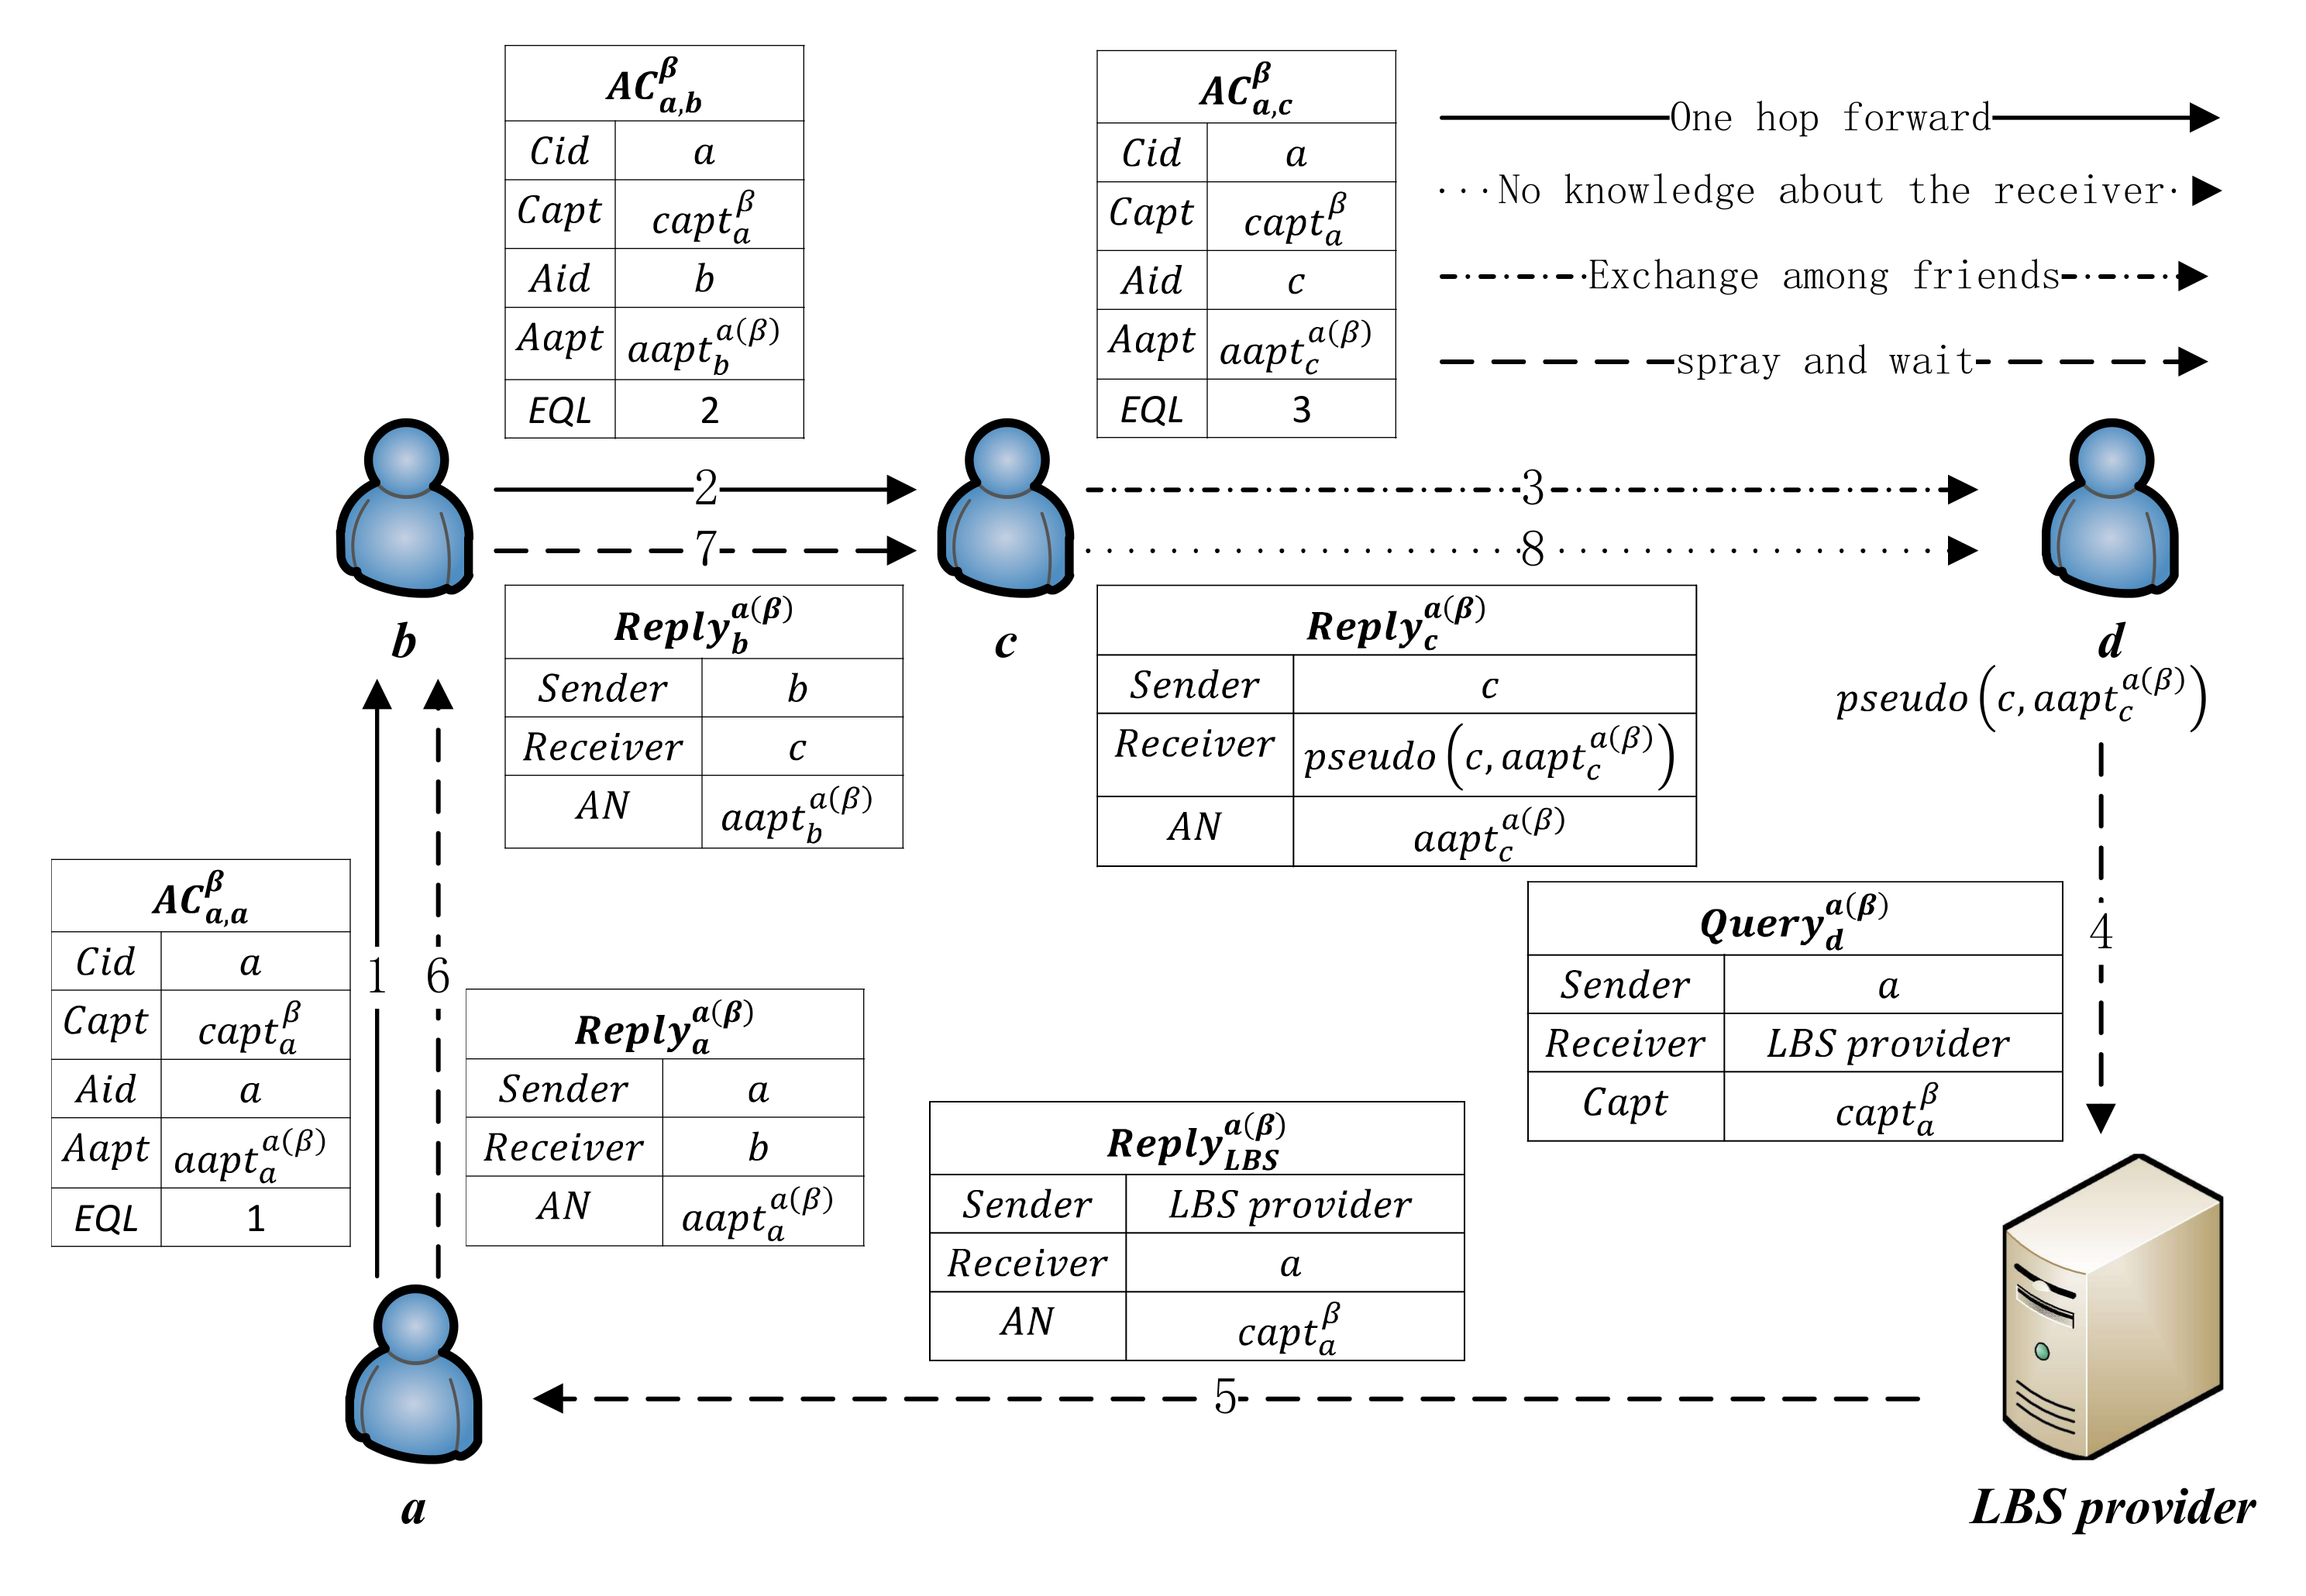
\includegraphics[width=6.0in]{figures/FIG_4_1_Example_of_ACP_Message_Exchange.png}
  \caption{Example of ACP Message Exchange} 
  \label{fig:EoACPME} %% label for entire figure 
\end{figure}


The Figure \ref{fig:EoACPME} is an example of the execution of the ACP protocol. Explanations of the symbols in the figure are shown in Table 4.1. These symbols and the figure are used throughout the chapter to help us describe the protocol. For simplicity, we will omit some superscripts and subscripts from these symbols in the following sections when there is no ambiguity. The whole process can be considered as the following parts: 1) exchanging cards among all users who are called agents (i.e., 1 and 2), 2) exchanging cards among friends (i.e., 3), 3) sending query using information of appointment cards (i.e., 4), 4) forwarding the reply among agents (i.e., 5, 6 and 7), and 5) relaying to the original requester (i.e., 8). 

\section{ Appointment Card}

\noindent Since the original requester cannot use his own identity to communicate with the LBSP, he must use others' identity (${Agt}_1$) to send queries, so that the LBSP can reply to the original requester through ${Agt}_1$. Appointment cards make it possible for the agents to forward the reply to the original requester one by one. In other words, the appointment card indicates a path through which the original requestor can get its reply. 

In Figure 4.1, the users \textit{a}, \textit{b} and \textit{c} are the agents of the appointment card ${AC}^{\beta }_a$ (i.e., ${Agt}^{a\left(\beta \right)}_1$, ${Agt}^{a\left(\beta \right)}_2$and ${Agt}^{a\left(\beta \right)}_3$). These agents are strangers, so the attackers can hardly infer $c$ from the identity of $a$. At the same time, $c$ is in the original requester $d$'s social tie (i.e.,$\ c$ is $d$'s friend or his friends' friend, so on), and he is the only one who knows how to reach $d$. Therefore, it is hard for attackers to infer the identity of $d$ from the identity of $a$.

Notice that $c$ receives $a$'s appointment card (i.e. ${AC}^{\beta }_a$) from a stranger $b$ who knows the information of ${AC}^{\beta }_a$ and the identity of the next agent $c$, so that it is unsafe for $c$ to use that appointment card. In other words, the appointment card cannot be used until $c$ exchanges it with another user (e.g., the user $d$) who trusts $c$. The appointment card is called a \textit{ready appointment card} (\textit{ready AC}) after it leaves the last agent (i.e., the user $c$), or it is called the \textit{distributing appointment card} (simply \textit{distributing AC}). It is obvious that \textit{distributing AC}s are transmitted among agents who can be strangers, while a user can only get \textit{ready AC}s from  one of his friends.

To make users carry a similar number of ready ACs, ready ACs are also exchanged between friends. As a result, the last agent is not sure whether the user who gets the ready AC from him is the original requester. We introduce a pseudonym mechanism, which enables the last agent to forward the reply to an unknown original requester. 

All users in the network are responsible for generating their respective ACs, and they are called the creators of their own ACs. The creator records his own identity ($Cid$) and a unique number ($Capt$) on his AC. When users exchange ACs, they modify $Aid$ (the agent ID) and $\mathrm{Aapt}$ (the agent's appointment number) in the AC to enable the next agent to identify who is the predecessor. Entries of AC are shown in Table 4.2.


\section{ AC Life Cycle}

\noindent The life cycle of an AC starts when it is generated by its creator. The first $k$ (see Table 4.3) agents add their identities into its Exchange Queue (EQ) (see Table 4.2) before exchanging it, which increases the length (\textit{EQL}) of the EQ. When the AC's \textit{EQL} reaches $k$, it is eligible to be used in a query and is called a \textit{ready }AC. When an AC is used in a query, it is marked as an \textit{used AC} by the original requester who uses the AC. No matter what state (\textit{distributing}, \textit{ready} or \textit{used}) an AC is in, it can expire, as shown in the Figure 4.2. An AC starts at the \textit{distributing} state. If the length of its \textit{EQ} reaches \textit{k}, it is switched to the \textit{ready} state. It can timeout in all states. If an AC is used once, it is switched to the \textit{used} state. A \textit{used} AC can also be used in other queries but cannot be given to anyone. 

\section{ System Parameters}

\noindent All the system parameters are shown in Table 4.3. 


\subsection{ Obfuscation Distance}

\noindent The obfuscation distance $k$ is the number of exchange before an AC is switched to the \textit{ready} state. In other words, an AC must be exchanged $k$ times before it becomes a \textit{ready} AC.

As shown in Figure 4.3, an AC is exchanged along ${Agt}_1$, ${Agt}_2$, ..., ${Agt}_k$. Since those agents are strangers, the only relationship between two adjacent agents is that they encounter each other somewhere. The relationship between ${Agt}_1$ and ${Agt}_k$ becomes weaker when we increase $k$. In other words, attackers can hardly infer the identity of ${Agt}_k$ when he only knows the identity of ${Agt}_1$, and his difficulty increases with the increase of parameter $k$. As a result, it is hard for attackers to infer the original requester, even though ${Agt}_k$ is in the social tie of the original requester. Since the reply message must go through a series of agents, a long obfuscation distance also lengthens the path of the reply message. Therefore, a large $k$ makes the original requester safer, while making it harder and longer for the reply to be delivered.


\subsection{ Friends Obfuscation Distance}

\noindent Since ${Agt}_{k-1}$ is a stranger for ${Agt}_k$, it is possible that ${Agt}_{k-1}$ is exactly the attacker. We assume that the attacker knows that ${Agt}_k$ is in the social tie of the original requester. The attacker can assume that ${Agt}_k$ is a close friend of the original requester, so the identity of ${Agt}_k$ gives the attacker a good tip to infer the original requester. A solution to prevent the agent ${Agt}_{k-1}$ from learning the original requester easily is that the last $m$ agents are friends, as shown in Figure 4.4. Here, $m$ is called \textit{friends obfuscation distance}, and the last $m$ agents are trusted agents.

It is true that ${Agt}_i$ is a friend of ${Agt}_{i+1}$, $i>k-m$, but two nonadjacent trusted agents (e.g., ${Agt}_i$ and ${Agt}_{i+2}$) might have a weak relationship. Since there are at least $m$ trusted agents between the stranger ${Agt}_{k-m}$ and the original requester, ${Agt}_{k-m}$ can hardly infer the identity of the original requester based on information he learns. When $m=k$, all ACs must be exchanged between friends only. When $m=1$, the last agent is the only one who is in social tie of the original requester, which is the case in our example.

However, friends encounter each other rarely, so having a large \textit{m} increases the difficulty of distributing ACs. In this work, we assign $m$ to 1.



\subsection{ Distributing Segment}

\noindent We again use the example in Figure 4.1. $U_a$ generates 3 ACs (i.e. ${AC}^1_a$, ${AC}^2_a$ and ${AC}^3_a$). It exchanges these ACs with $U_b$, then $U_b$ exchanges them with $U_c$ and so on. At last, all of them reach the original requester $U_d$. In this case, $U_d$ has several ACs whose paths (the list of agents) are the same, so $U_d$ has no choice but to choose one. In other words, since using these ACs results in the same reply path, $U_d$ is can simply choose an AC based on specific requirement it might have (e.g. the number of possible encounters of an agent). 

If agents exchange ACs with different users, the above problem will not happen. We use the system parameter distributing segment, $Seg$, to avoid giving all ACs to the same user. Each user maintains $Seg$ number of \textit{Distributing AC List}s (\textit{DL}s). It puts received \textit{distributing} ACs in one of those \textit{DL}s randomly. If ${Agt}_i$ exchanges ACs with another user, ${Agt}_i$ selects one of his \textit{DL}s, and only ACs in that \textit{DL} will be exchanged with that user.

For example, we assign $Seg=2$ so that each user has two \textit{DL}s (i.e., \textit{DL}1 and \textit{DL}2). When $U_b$ receives ${AC}^1_{a,a}$, ${AC}^2_{a,a}$ and ${AC}^3_{a,a}$ from $U_a$, $U_b$ may put ${AC}^1_{a,a}$ and ${AC}^2_{a,a}$ in its \textit{DL}1, while ${AC}^3_{a,a}$ in its \textit{DL}2. If $U_b$ encounters $U_c$, $U_b$ can give either ${AC}^1_{a,b}$ and ${AC}^2_{a,b}$ or only ${AC}^3_{a,b}$ to $U_c$. In this way, we separate ACs generated by the same creator.


\subsection{ Generating Period}

\noindent Since ACs could expire, users must generate new ACs continuously. We use GP to denote the speed of generating new ACs per user, that is, each user generates a new AC every GP seconds.


\subsection{ AC Timeout}

\noindent Let $AT$ denote the timeout of ACs. An AC expires $AT$ seconds after it is generated. When an AC expires, all agents delete the AC information from their memory.


\subsection{ Avoiding Time}

\noindent If a user gets an AC at time $t_i$, he cannot get that AC again before $t_i+\tau $, where $\tau$ is parameter avoiding time. The reason for this is described in Section 4.6.2.


\section{ Protocol Details}


\subsection{ Generating Appointment Cards}

\noindent Maintaining a certain number of ACs in the network is a prerequisite for users for sending queries. Considering that ACs can expire, users must generate ACs continuously. The user who generates an AC is called the creator of the AC, at the same time, he is also the first agent of the AC. ACs are generated based on two principles: fairness and continuity. 

ACs impose burden on agents. In fact, agents are unlikely to benefit from relaying messages to the original requester because they need to allocate memory to save ACs' information, and they consume energy to forward replies. To prevent users who generate more ACs than others being overloaded, some fairness mechanism must be in place to ensure that all users generate a fairly equal number of ACs.

We assume that the AC timeout (i.e. $AT$) is 30 minutes, and every user generates 100 ACs at the beginning and generates no AC until the 30${}^{th}$ minute. Since all agents remove the information of expired ACs from their memory, a reply can hardly be delivered when the AC it uses is timed out (expired). As a result, it is hard for a user to select an appropriate AC for his query at the 29${}^{th}$ minute when all ACs only have 1 ($=30-29$) more minute, because his reply may be lost even though his query is delivered successfully. Therefore, the generating strategy should be a steady and sustainable.

In our protocol, each user generates a new AC every GP second. Since an AC has an AT-seconds timeout, there are about $\delta =\frac{AT}{GP}$ appointment cards hold by each user in the network. In other words, each user maintains about $\delta$ ACs which is generated by himself, and we meet the fairness criteria. Since users generate ACs continuously, ACs have various timeouts so that it is likely for a user to pick an AC who does not expire in a long time (at least longer than his queries and replies).


\subsection{ Exchange Distributing Appointment Cards}

\noindent Users exchange their \textit{distributing} ACs as frequently as possible, so that a \textit{distributing} AC can be switched to a \textit{ready} one quickly. Still, there are some other conditions which should be satisfied when exchanging a \textit{distributing} AC.

We assume that two users, e.g. $U_A$ and $U_B$, are walking together for a some time. Also assume that $U_A$ generates an AC (e.g., ${AC}_A$) at $t_0$ and exchanges it to $U_B$, then ${AC}_A$ is given back to A and so on. The distributing phase of the AC only costs a few seconds, because $U_A$ and $U_B$ are the only agents involved. This defeats the purpose of exchanging ACs, because it is easy for an attacker to infer the last agent who may be $U_A$ or $U_B$ from the first agent $U_A$. 

We use a parameter \textit{avoiding time,} $\tau$, to optimize the agent selection strategy. If a user gets an AC at time $t_i$, he cannot get that AC again before $t_i+\tau $. For example, $U_B$ receives a certain AC ${AC}_A$ from $U_A$ at $t_0$, then $U_B$ sends it to a user C ($U_C$) who can also send it to others. If a user carrying ${AC}_A$ encounters $U_B$  before $t_0+\tau $, he cannot send ${AC}_A$ to $U_B$. Therefore, if the parameter $\tau $ is larger than or equal to the parameter \textit{AT}, there is no repeated agent in an AC's EQ. In other words, an AC never reaches an agent twice when $\tau $ is equal to \textit{AT}. In this thesis, we assign $\tau $ to \textit{AT}. 

Besides, we should also avoid ACs having the same sequence of agents, as we mention in the distributing segment subsection. Now we propose the strategy of exchanging distributing ACs.

Let us take a pair of users Alice and Bob as an example. If Alice encounters another user Bob, Bob tells Alice whether he trusts her (she is viewed as a friend by Bob). Alice picks one of her distributing AC lists (e.g. \textit{DL}1). Alice traverses all ACs in \textit{DL}1, and distributing ACs which satisfy the following two conditions before exchanging them with Bob.

\begin{enumerate}
\item  If the length of the AC's EQ (i.e. EQL) is not shorter than $k-m$, then Alice must be a friend of Bob.

\item  Bob was not carrying the AC in the recent $\tau $ time interval.
\end{enumerate}

When Alice sends a distributing AC to Bob, she adds her identity and current time to the AC's EQ. Besides, Alice must modify the AC's $Aid\mathrm{\ }$to her own identity and its $Aapt$ to a new one. The information in Table 4.4 is recorded as \textit{relay table} in her memory. We should notice that the first agent (i.e., the creator) does not have a ${Aapt}_{old}$, because he is precisely the one who has generated the AC, in which case the ${Aapt}_{old}$ indicates his own identity. When Bob gets those ACs, he puts each one of the received \textit{distributing} ACs to his \textit{DL}s respectively and randomly. If an AC whose EQL is already equal to $k$, the AC must be switched to a \textit{ready} one when Bob gets it. Bob puts ready ACs in his ready AC list instead of distributing AC lists.

Table 4.4: Relay Table Entries

\begin{tabular}{|p{1.2in}|p{3.0in}|} \hline 
Name of entries & descriptions \\ \hline 
${Aapt}_{old}$ & The $Aapt$ generated by the previous agent \\ \hline 
${Aid}_{old}$ & The identity of the previous agent \\ \hline 
${Aapt}_{new}$ & The new $Aapt$ (generated by himself) \\ \hline 
${ID}_{nxt}$ & The identity of the next agent \\ \hline 
$EQL$ & The length of the AC's EQ (should larger than 0) \\ \hline 
$AT$ & The time when the AC timeout. \\ \hline 
\end{tabular}

\subsection{ Exchange Ready Appointment Cards}

\noindent Users ask for ready ACs only from their friends, which ensures that the information of the ready ACs held by a user is not exposed to strangers. The strategy of exchanging ready ACs should also meet some fairness criteria. That is, the number of each user's ready ACs should be more or less equal. 

Let us consider two friends Alice and Bob as an example. Alice has 20 ACs, while Bob has 10 ACs. When they encounter each other, it is reasonable that they both give half of their ready ACs to the other. As a result, they both will have half of the total \eqref{GrindEQ__15_} ACs. However, that strategy does not work all the time as explained below.

The problem becomes more complex in the following condition. Alice is a friend of Bob, while Bob is not a friend of Alice. In other words, Bob trusts Alice, but Alice does not trust Bob. We assume that Alice is a trusted but suspicious girl so that many users trust her while she trusts few users while Bob is opposite. When users encounter Alice, they ask for ready ACs from her, but Alice rarely asks for ready ACs. Therefore, Alice carries few ready ACs, while Bob carries many ready ACs. When Alice and Bob encounter each other, it is Bob who is asking for ready ACs instead of Alice. To make the strategy fair and efficient, users must compare the number of their own ready ACs and the number of ready ACs carried by the other user when two users are exchanging ready ACs.

When Bob encounters Alice, Bob tells Alice the number of his ready ACs (${NR}_{Bob}$) and whether he wants Alice's ready ACs (if he trusts Alice). If Alice learns that Bob needs her ready ACs, she compares the number of her ready ACs (${NR}_{Alice}$) and ${NR}_{Bob}$. If ${NR}_{Bob}\ge {NR}_{Alice}$, Alice gives no ready AC to Bob; otherwise, she gives $\frac{{NR}_{Alice}-{NR}_{Bob}}{2}$ to Bob. In this way, ready ACs do not concentrate in a group of users who trust many users. 

The process of exchanging ready ACs is much simpler than that for distributing ACs. Users do not modify any information in the ready ACs including $Aapt$ and $Aid$, so that ready ACs do not change after they leave the last ($k^{th}$) agent.

The algorithm of exchanging ACs when a user $U_i$ encounters another user $U_j$ is shown in Algorithm 4-1. The two users tell the other whether they are friends at the very beginning of their encounter. After they both know their relationship, they start to exchange their distributing ACs. When they both finish receiving the distributing ACs from the other, they continue to exchange their ready ACs at the same time. The process ends when they finish exchanging their ready ACs (or they do not need to exchange ready ACs).

\subsection{ Sending Queries}

\noindent For an original requester who want to send queries to the LBSP, his query must be delivered to the LBSP while the LBSP cannot learn the identity of him. Besides, the reply message from the LBSP must be delivered back to the original requester. The basic idea is that the original requester sends his query using another user's identity to the LBSP, so that LBSP can reply to that user who is responsible to forward the reply to the original requester. That user is the first agent ($Agt_1$) of the AC which is used by the queries of the original requester.

In order to enable LBSP to reply to ${Agt}_1$, the original requester's query includes an sender identity ${Agt}_1$, which is equal to the $Cid$ in the AC. Since ${Agt}_1$ needs a $\mathrm{Capt}$ to identify the AC used by the query (and the reply), the $\mathrm{Capt}$ in the AC is also in the query. The network can deliver that query to the destination LBSP easily with any DTN protocols.

We use the example in Figure 4.1. The original requester $U_d$ has an AC (i.e., ${AC}^{\beta }_{a,c}$) whose creator is $U_a$. When $U_d$ uses it to send his query ${Query}^{a\left(\beta\right)}_d$, the sender identity is $a$ and the $Capt$ of the query is the $Capt$ of ${AC}^{\beta }_{a,c}$, as shown in Figure 4.5.

The AC is marked as used when the query is ready to be sent, so that the AC cannot be exchanged to other users. To get the reply, the original requester also uses a pseudonym, which is described later. The algorithm that a user $U_i$ sends a query is shown in Algorithm 4-2.


\subsection{ Sending Replies}


\subsubsection{ The LBSP part}

\noindent When the LBSP received the query, it learns that the sender's identity is the first agent instead of the original requester, which protects the location privacy of the original requester. The LBSP reply to the first agent using the information in the query.

Figure 4.6: Constitute Replies

\noindent In Figure 4.6, the LBS provider reply to the sender $U_a$, when it receives ${Query}^{a\left(\beta\right)}_d$. The $Capt$ of the query is also included in the reply, which enables $U_a$ to identify the AC used in the query and the reply.


\subsection{ The First Agent}

\noindent When the first agent (i.e. ${Agt}_1$) gets the reply from the LBSP, he learns the $\mathrm{AN}$ in the reply. He searches his reply table to get the information of the AC used in the query and reply. If the AC does not expire, there must be a corresponding entry in his reply table, as shown in Table 4.5. ${Agt}_1$ gets an entry where the $Aid_{old}$ and ${Aapt}_{old}$ are equal to his identity and the $AN$ of the reply. As a result, he learns the identity of the next agent (i.e. ${Agt}_2$) from the ${ID}_{nxt}$ of the entry, so ${Agt}_1$ forwards the reply to ${Agt}_2$. The $AN$ of the reply is replaced with the ${Aapt}_{new}$ in the entry by ${Agt}_1$, which enables ${Agc}_2$ to identify the AC in ${Agt}_2$'s reply table.

\noindent 

Table 4.5: Reply Table Entries Of The First Agent

\begin{tabular}{|p{1.0in}|p{2.4in}|} \hline 
Name of entries & value \\ \hline 
${Aid}_{old}$ & The user's own identity \\ \hline 
${Aapt}_{old}$ & The $Capt$ of the AC used in the reply (query) \\ \hline 
${ID}_{nxt}$ & The identity of the second agent \\ \hline 
${Aapt}_{new}$ & The $Aapt$ given to the second agent by the user. \\ \hline 
$EQL$ & $1$ \\ \hline 
$AT$ & The time when the AC timeout. \\ \hline 
\end{tabular}

For the example in Figure 4.1, the first agent is $U_a$. When he receives ${Reply}^{\mathrm{a}\left(\beta\right)}_{LBS}$, he learns that it is a reply from the LBS and the $Capt$ of the AC is ${capt}^{\beta}_a$. He searches his reply table for an entry whose ${Aid}_{old}$ is equal to $a$ and ${Aapt}_{old}$ is equal to ${capt}^{\beta }_a$. As shown in Figure 4.7, the ${ID}_{nxt}$ in the entry is equal to $b$ so he modifies the receiver of the reply message to $U_b$. $U_a$ also modifies the $AN$ in the reply message to ${aapt}^{a\left(\beta\right)}_a$ which enables $U_b$ identifies the AC in his reply table, because the ${Aapt}_{new}$ in the entry is equal to ${aapt}^{a\left(\beta\right)}_a$. 

Figure 4.7: The Reply of The First Agent


\subsection{ Intermediate Agents}

\noindent The process of forwarding replies in the intermediate agents (the second to the ${\left(k-1\right)}^{th}$ one) is similar with that of the first agent. We take the second agent as an example. When the second agent receives the reply forwarded by the first one, he learns the sender's identity (i.e. the first agent) and the $AN$ from the reply. Since he gets the AC which is used in the reply (query) from the previous agent, there must be an entry, whose ${Aid}_{old}$ is equal to the previous agent's identity and the ${Aapt}_{old}$ is the value of $Aapt$ in the AC when he gets it, in his reply table, as shown in Table 4.6.


Table 4.6: Reply Table Entries Of The Second Agent

\begin{tabular}{|p{1.0in}|p{2.5in}|} \hline 
Name of entries & value \\ \hline 
${Aid}_{old}$ & The identity of the previous agent (i.e. the first agent) \\ \hline 
${Aapt}_{old}$ & The $Aapt$ given by the previous agent. \\ \hline 
${ID}_{nxt}$ & The identity of the next agent (e.g. the third agent) \\ \hline 
${Aapt}_{new}$ & The $Aapt$ given to the next agent by the user. \\ \hline 
$EQL$ & 2 \\ \hline 
$AT$ & The time when the AC timeout. \\ \hline 
\end{tabular}

For the example in Figure 4.1, the second agent is $U_b$. When he receives ${Reply}^{a\left(\beta\right)}_a$, he learns that it is $U_a$ who forwards the reply message ${Reply}^{a\left(\beta\right)}_a$ and the $Aapt$ of the AC is ${aapt}^{a\left(\beta\right)}_a$. He searches his reply table for an entry whose ${Aid}_{old}$ is equal to $a$ and ${Aapt}_{old}$ is equal to ${aapt}^{a\left(\beta\right)}_a$. As shown in Figure 4.8, since the ${ID}_{nxt}$ in the entry is equal to $c$, he modifies the receiver of the reply message to $U_c$. $U_b$ also modifies the $AN$ in the reply message to ${aapt}^{a\left(\beta\right)}_b$ which enables $U_c$ identifies the AC in his reply table, because the ${Aapt}_{new}$ in the entry is equal to ${aapt}^{a\left(\beta\right)}_b$. 

Figure 4.8: The Reply of the Second Agent

For each agent ${Agt}_i$, where $2\le i\le k-1$, he searches his reply table for a correlative entry, when he receives a reply. The ${Aid}_{old}$ and ${Aapt}_{old}$ in the entry should be equal to the sender's identity and the $AN$ in the reply. The identity of the next agent ${Agt}_{i+1}$ is ${ID}_{nxt}$. ${Agc}_i$ also assign ${Aapt}_{new}$ to the $AN$ in the reply to help ${Agt}_{i+1}$ search ${Agt}_{i+1}$'s reply table.

\subsection{ The Last Agent}

\noindent The last agent also searches for a reply table entry based on the reply, while he cannot get the identity of the next agent. The reply table entry of the last agent is shown in Table 4.7.

The last agent uses the same way to look up an entry in his reply table as the previous agents. When he finds that the $EQL$ is equal to $k$, he notices that he is the last agent. Then he is responsible to forward the reply to the original requester instead of another agent. He uses his identity and ${Aapt}_{new}$ in his reply table entry to generates a pseudonym $pseudo\left({Agc}_k,{Aapt}_{new}\right)$, where the function $pseudo\left(id,Aapt\right)$ is a public pseudonym generating function which everyone in the network knows, including the original requester.

When the original requester sends his query, he also gets the same pseudonym $pseudo\left({Agc}_k,{Aapt}_{new}\right)$ using the pseudonym generating function. Note that he can get parameters from the AC. ${Agc}_k$ and ${Aapt}_{new}$ are equal to the $Aid$ and $Aapt$ in the AC. He uses that pseudonym as his identity before he gets the reply.

When users deliver the reply from the last agent, they are looking for a user whose identity is that pseudonym. At last, the original requester gets the reply, because he is the only user who uses the pseudonym as his identity.

For the example in Figure 4.1, the last agent is $U_c$. When he receives ${Reply}^{a\left(\beta\right)}_b$, he learns that it is $U_b$ who forwards the reply message ${Reply}^{a\left(\beta\right)}_b$ and the $Aapt$ of the AC is ${aapt}^{a\left(\beta\right)}_b$. He searches his reply table for an entry whose ${Aid}_{old}$ is equal to $b$ and ${Aapt}_{old}$ is equal to ${aapt}^{a\left(\beta\right)}_b$. Since the $EQL$ in the entry is equal to 3 (i.e. $k$), he recognizes that he is the last agent. $U_c$ calculates the pseudonym ${psd}^{a\left(\beta \right)}_c=pseudo\left(c,{aapt}^{a\left(\beta\right)}_c\right)$ then forward the reply to ${psd}^{a\left(\beta\right)}_c$. The original requester $d$ gets the identity $c$ and the ${aapt}^{a\left(\beta \right)}_c$ from the AC he uses, so that he uses the pseudonym ${psd}^{a\left(\beta \right)}_c$ as his identity. As a result, $U_d$ get the reply from $U_c$. The $AN$ of the reply is also assigned to ${aapt}^{a\left(\beta\right)}_c$ to avoid identical pseudonyms. The process is shown in Figure 4.9. 


\section{ Appointment Number}

\noindent The Appointment Number (AN) including $Capt$ and $Aapt$ is significant information in the AC. We explain the rules of generating them in detail and talk about the effect of ACs' timeout mechanism in this section.


\subsection{  Creator Appointment Number}

\noindent The Creator Appointment Number ($Capt$) is a number which is used to identify ACs generated by the same creator. In other words, if two ACs are generated by the same creator and they do not expire, their $Capt$ must be different. Therefore, the first agent (i.e., the creator) cannot find two entries which have the same ${Aapt}_{old}$ in his reply table, if their ${Aid}_{old}$ are both his own identity.


\subsection{ Agent Appointment Number}

\noindent The Agent appointment number ($Aapt$) is a number used to identify appointment cards who have the same agent. Agents generate a new $Aapt$s for appointment cards before they exchange those cards to others. In other words, an agent gives any appointment card passing on by him a unique $Aapt$, which helps the next agent identify the appointment card in his reply table. Since the $Aapt$ is unique, an agent who is not the first one cannot find two entries which have the same pair of ${Aid}_{old}$ and ${Aapt}_{old}$, neither.


\subsection{ Timeout}

\noindent Agents delete the entries, which contains the information of expired ACs, from his reply table. Consequently, agents cannot forward replies using ACs which expire before this very moment. That is the reason why an original requester must choose a AC which expires after his query and reply timeout. While the timeout mechanism has more advantage than disadvantage.

Since users are moving, the distance between agents and the original requester might be too large after a long time. As a result, it is hard for agents to forward the reply messages back to the original requester, so that the original requester takes a higher risk when he uses an AC which is generated for a long time. Then these kind of ACs might not be used after a period, while it cost agents a few memories to save the ACs' information in their reply table. Therefore, all users remove the information of expired ACs to save their memories.

We should also notice that an unexpired AC and an expired one might have the same $Capt$ or $Aapt$. Because no agent keeps the record of the expired AC, so that the duplication cannot confuse agents.




































